\section{Faithful progress measures (Nanda et al.)}
\label{app:progress}

For logits $L_{a,b,c}$ over all $(a,b,c)\in\{0,\ldots,P{-}1\}^3$, we define restricted (trigonometric) and excluded loss on the full $P^3$ logit grid following \citet{nanda2023progress}.

\section{Checkpoint selection}
\label{app:checkpoints}

For each seed we select three checkpoints from the logged training history:
\textbf{Final} (last logged step),
\textbf{Grokking} (first step with test accuracy $\geq 0.99$ and test loss $\leq 0.05$),
\textbf{Best FVE} (highest faithful trig-FVE among steps with test accuracy $\geq 0.99$).
Full TRM mechanistic analysis uses grokking/best-FVE when final checkpoints degrade.

\begin{tabular}{llrr}
\toprule
Model & Checkpoint & Test Acc. & Faithful FVE \\
\midrule
nanda\_a\_mlp & Final & 1.000 $\pm$ 0.000 & 0.827 $\pm$ 0.045 \\
nanda\_a\_mlp & Grokking & 1.000 $\pm$ 0.001 & 0.349 $\pm$ 0.428 \\
nanda\_a\_mlp & Best FVE & 0.999 $\pm$ 0.001 & 0.888 $\pm$ 0.023 \\
trm\_full\_a & Final & 0.811 $\pm$ 0.374 & 0.393 $\pm$ 0.071 \\
trm\_full\_a & Grokking & 0.998 $\pm$ 0.001 & 0.000 $\pm$ 0.000 \\
trm\_full\_a & Best FVE & 0.999 $\pm$ 0.002 & 0.449 $\pm$ 0.051 \\
trm\_full\_b & Final & 0.953 $\pm$ 0.091 & 0.187 $\pm$ 0.127 \\
trm\_full\_b & Grokking & 0.996 $\pm$ 0.002 & 0.048 $\pm$ 0.095 \\
trm\_full\_b & Best FVE & 0.995 $\pm$ 0.004 & 0.298 $\pm$ 0.117 \\
trm\_minimal & Final & 1.000 $\pm$ 0.000 & 0.509 $\pm$ 0.339 \\
trm\_minimal & Grokking & 0.997 $\pm$ 0.003 & 0.293 $\pm$ 0.384 \\
trm\_minimal & Best FVE & 1.000 $\pm$ 0.000 & 0.786 $\pm$ 0.158 \\
\bottomrule
\end{tabular}


\section{Per-seed metrics}
\label{app:perseed}

Table~\ref{tab:perseed} lists every seed with final, grokking, and best-FVE metrics plus automated variance diagnosis.

\footnotesize
\setlength{\tabcolsep}{4pt}
\begin{longtable}{llrrrrrr p{2.4cm}}
\caption{Per-seed metrics and diagnosis.}\label{tab:perseed} \\
\toprule
Model & Seed & Final Acc & Final FVE & Grok Step & Grok FVE & Best Step & Best FVE & Diagnosis \\
\midrule
\endfirsthead
\multicolumn{9}{c}{\tablename\ \thetable\ -- continued} \\
\toprule
Model & Seed & Final Acc & Final FVE & Grok Step & Grok FVE & Best Step & Best FVE & Diagnosis \\
\midrule
\endhead
nanda\_a\_mlp & 0 & 1.000 & 0.827 & 3100 & 0.000 & 3000 & 0.883 & stable\_\allowbreak circuit \\
nanda\_a\_mlp & 1 & 1.000 & 0.747 & 4100 & 0.000 & 4000 & 0.849 & stable\_\allowbreak circuit \\
nanda\_a\_mlp & 2 & 0.999 & 0.848 & 3100 & 0.000 & 37000 & 0.916 & stable\_\allowbreak circuit \\
nanda\_a\_mlp & 3 & 1.000 & 0.884 & 4000 & 0.878 & 48000 & 0.903 & stable\_\allowbreak circuit \\
nanda\_a\_mlp & 4 & 1.000 & 0.829 & 5000 & 0.867 & 5500 & 0.890 & stable\_\allowbreak circuit \\
trm\_full\_a & 0 & 1.000 & 0.408 & 4700 & 0.000 & 9500 & 0.443 & stable\_\allowbreak circuit \\
trm\_full\_a & 1 & 0.996 & 0.514 & 6100 & 0.000 & 6000 & 0.514 & stable\_\allowbreak circuit \\
trm\_full\_a & 2 & 0.063 & 0.383 & 5400 & 0.000 & 6500 & 0.401 & incomplete\_\allowbreak grokking\_\allowbreak by\_\allowbreak 20k \\
trm\_full\_a & 3 & 0.996 & 0.295 & 6900 & 0.000 & 7500 & 0.388 & cleanup\_\allowbreak phase\_\allowbreak fve\_\allowbreak collapse \\
trm\_full\_a & 4 & 1.000 & 0.364 & 8200 & 0.000 & 8500 & 0.501 & cleanup\_\allowbreak phase\_\allowbreak fve\_\allowbreak collapse \\
trm\_full\_b & 0 & 1.000 & 0.093 & 4100 & 0.000 & 39000 & 0.220 & cleanup\_\allowbreak phase\_\allowbreak fve\_\allowbreak collapse \\
trm\_full\_b & 1 & 1.000 & 0.377 & 18000 & 0.238 & 33000 & 0.445 & cleanup\_\allowbreak phase\_\allowbreak fve\_\allowbreak collapse \\
trm\_full\_b & 2 & 0.993 & 0.082 & 7300 & 0.000 & 46500 & 0.437 & cleanup\_\allowbreak phase\_\allowbreak fve\_\allowbreak collapse \\
trm\_full\_b & 3 & 0.772 & 0.304 & 3400 & 0.000 & 37500 & 0.186 & incomplete\_\allowbreak grokking\_\allowbreak by\_\allowbreak 20k,\allowbreak cleanup\_\allowbreak phase\_\allowbreak fve\_\allowbreak collapse \\
trm\_full\_b & 4 & 1.000 & 0.082 & 8900 & 0.000 & 27500 & 0.204 & cleanup\_\allowbreak phase\_\allowbreak fve\_\allowbreak collapse \\
trm\_minimal & 0 & 1.000 & 0.937 & 4500 & 0.947 & 5000 & 0.962 & stable\_\allowbreak circuit \\
trm\_minimal & 1 & 1.000 & 0.907 & 9400 & 0.000 & 46500 & 0.909 & stable\_\allowbreak circuit \\
trm\_minimal & 2 & 1.000 & 0.198 & 14700 & 0.000 & 15000 & 0.642 & cleanup\_\allowbreak phase\_\allowbreak fve\_\allowbreak collapse \\
trm\_minimal & 3 & 1.000 & 0.272 & 9400 & 0.000 & 9500 & 0.858 & cleanup\_\allowbreak phase\_\allowbreak fve\_\allowbreak collapse \\
trm\_minimal & 4 & 1.000 & 0.228 & 19000 & 0.518 & 19500 & 0.558 & post\_\allowbreak grokking\_\allowbreak fve\_\allowbreak decay,\allowbreak cleanup\_\allowbreak phase\_\allowbreak fve\_\allowbreak collapse \\
\bottomrule
\end{longtable}
\normalsize


\section{TRM minimal seed variance}
\label{app:variance}

Post-grokking cleanup (weight decay removing memorizing components) can collapse faithful FVE while test accuracy remains high---mirroring Nanda's cleanup phase but with higher seed variance in TRM minimal.

\begin{adjustbox}{max width=\linewidth}
\begin{tabular}{rrrrr p{4cm}}
\toprule
Grok Step & Peak FVE & Peak Step & Final FVE & FVE Drop & Cause \\
\midrule
4500 & 0.962 & 5000 & 0.937 & 0.025 & stable\_\allowbreak circuit \\
9400 & 0.909 & 46500 & 0.907 & 0.002 & stable\_\allowbreak circuit \\
14700 & 0.701 & 14500 & 0.198 & 0.503 & cleanup\_\allowbreak phase\_\allowbreak fve\_\allowbreak collapse \\
9400 & 0.866 & 9000 & 0.272 & 0.594 & cleanup\_\allowbreak phase\_\allowbreak fve\_\allowbreak collapse \\
19000 & 0.558 & 19500 & 0.228 & 0.330 & post\_\allowbreak grokking\_\allowbreak fve\_\allowbreak decay,\allowbreak cleanup\_\allowbreak phase\_\allowbreak fve\_\allowbreak collapse \\
\bottomrule
\end{tabular}
\end{adjustbox}


\section{Grokking dynamics and progress measures}
\label{app:grokking}

Figure~\ref{fig:grokking_curves} shows train/test accuracy and loss across
training (delayed generalization), and Figure~\ref{fig:progress_measures} shows
the restricted (trigonometric) and excluded losses tracking the full loss
post-grokking, mirroring Figure~1 of \citet{nanda2023progress}.

\begin{figure}[h]
  \centering
  
\includegraphics[width=0.95\linewidth]{figures/fig_grokking_curves.pdf}
  \caption{Train/test accuracy and loss vs.\ step (TRM minimal seed~0).}
  \label{fig:grokking_curves}
\end{figure}

\begin{figure}[h]
  \centering
  
\includegraphics[width=0.95\linewidth]{figures/fig_progress_measures.pdf}
  \caption{Restricted, excluded, and full cross-entropy vs.\ step.}
  \label{fig:progress_measures}
\end{figure}

\section{Mechanistic circuit analysis}
\label{app:mechanistic}

We analyze $W_E$, $W_U$, logit-map DFT energy, $W_L$ neuron--logit maps, MLP neuron clustering ($R^2$ to $\cos/\sin(\omega_k(a+b))$), and attention routing.

\begin{figure}[h]
  \centering
  
\includegraphics[width=0.95\linewidth]{figures/fig_progress_trajectory.pdf}
  \caption{Progress measures across saved checkpoints (TRM minimal seed~0).}
  \label{fig:traj}
\end{figure}

\begin{figure}[h]
  \centering
  
\includegraphics[width=0.7\linewidth]{figures/fig_frequency_ablations.pdf}
  \caption{Causal key-frequency ablations at convergence.}
  \label{fig:abl}
\end{figure}

\begin{figure}[h]
  \centering
  
\includegraphics[width=0.95\linewidth]{figures/fig_mechanistic_circuit.pdf}
  \caption{Embedding and unembedding Fourier components.}
  \label{fig:mech}
\end{figure}

\section{Multi-seed robustness}
\label{app:seeds}

We train seeds $\{0,1,2,3,4\}$ for 50{,}000 steps; per-seed accuracy, best-FVE, and grokking curves appear in the main text (Figures~\ref{fig:multiseed} and~\ref{fig:multiseed_curves}).

\section{Combined phase plot (Nanda Fig.~7 style)}
\label{app:phase}

\begin{figure}[h]
  \centering
  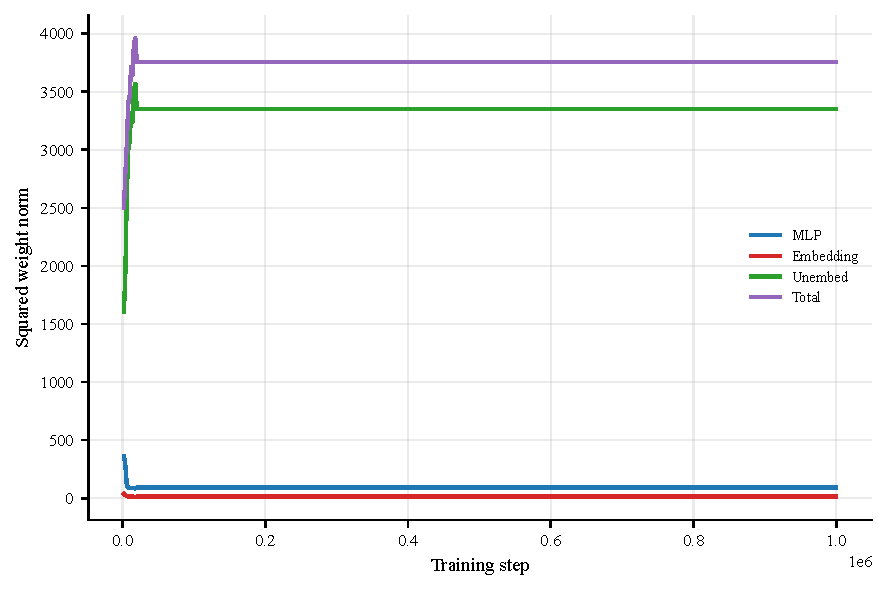
\includegraphics[width=0.85\linewidth]{figures/fig_weight_norm_phases.pdf}
  \caption{Weight-norm trajectory annotated with memorization, circuit-formation,
  and cleanup phases (\citealp{nanda2023progress}, Fig.~7 style).}
  \label{fig:weight_norm_phases}
\end{figure}

\section{Frequency ablations}
\label{app:ablations}

\begin{enumerate}
  \item \textbf{Trig (key):} retain only key-frequency components.
  \item \textbf{Excluded (key):} remove key components sequentially.
  \item \textbf{All-frequency grid:} retain/ablate each $k\in\{1,\ldots,P/2\}$ individually.
\end{enumerate}

The all-frequency ablation grid appears in the main text (Figure~\ref{fig:all_freq}).

\section{Hyperparameters}
\label{app:hparams}

\begin{table}[h]
  \centering
  \caption{Training hyperparameters (hybrid rigor, 50k steps).}
  \begin{tabular}{ll}
    \toprule
    Parameter & Value \\
    \midrule
    $P$ & 113 \\
    Train fraction & 0.3 \\
    Optimizer & AdamW \\
    Learning rate & $10^{-3}$ \\
    Weight decay & 1.0 \\
    $\beta_1, \beta_2$ & 0.9, 0.98 \\
    Steps & 50{,}000 \\
    Seeds & $\BMINSeeds$ \\
    Hidden size & 128 \\
    Heads & 4 \\
    ACT max steps & 8 (full TRM) \\
    \bottomrule
  \end{tabular}
\end{table}

\section{HRM / latent recursion probes}
\label{app:hrm}

Fixed-point violation rate, reasoning-mode counts, mean-field CE by ACT step, and ACT-depth ablations.

\section{Detailed progress-measure methodology}
\label{app:detailed_methods}

This appendix mirrors Section~5 of \citet{nanda2023progress} with TRM-specific implementation notes.

\subsection{Logit grid extraction}
For each pair $(a,b)$ in the modular-addition dataset, TRM receives input tokens $[a, b, \texttt{=}]$.
We run a single forward pass with ACT halted and read logits at position~2 (the ``$=$'' token).
Stacking over all $P^2$ pairs yields $L \in \mathbb{R}^{P \times P \times P}$ where $L_{a,b,c}$ is the logit for output $c$.

\subsection{Fourier basis on cyclic groups}
For prime modulus $P=113$, define $\omega_k = 2\pi k / P$.
Basis functions on index $x \in \{0,\ldots,P-1\}$:
\begin{align}
  \phi_k^{\cos}(x) &= \cos(\omega_k x), &
  \phi_k^{\sin}(x) &= \sin(\omega_k x).
\end{align}
For the logit map, the trigonometric identity $\cos(\omega_k(a+b-c))$ decomposes into products of 1D Fourier components along $a$, $b$, and $c$.

\subsection{Restricted (trigonometric) loss}
Given key frequencies $K = \{k_1,\ldots,k_5\}$, we project $L$ onto the span of $\cos(\omega_k(a+b))$ and $\sin(\omega_k(a+b))$ directions for $k \in K$, apply bias correction per \citet{nanda2023progress}, and compute cross-entropy against labels on train and test splits.

\subsection{Excluded loss}
For each $k \in K$ in descending sensitivity order, we subtract the rank-1 component associated with frequency $k$ from logits and measure test CE.
High excluded loss at step~2000 and low excluded loss at convergence indicate circuit formation.

\subsection{Embedding and unembedding Fourier norms}
$W_E \in \mathbb{R}^{P \times d}$: apply 1D DFT along the token axis (rows), sum $\ell_2$ energy per frequency pair $(k_{\cos}, k_{\sin})$.
$W_U \in \mathbb{R}^{P \times d}$: same along the vocabulary axis of the output head.
Key frequencies are those with largest excluded-loss sensitivity (not simply largest embedding norm).

\subsection{Gini coefficient}
Following Nanda Appendix~B, we compute the Gini coefficient of the vector of embedding Fourier norms to track sparsification during grokking.

\section{Reverse-engineering methodology}
\label{app:reverse_methods}

\subsection{$W_L$ neuron-logit map}
For SwiGLU layer $\ell$ with down-projection $W_{\mathrm{down}}^{(\ell)} \in \mathbb{R}^{d \times d_{\mathrm{ff}}}$ and unembedding $W_U \in \mathbb{R}^{P \times d}$:
\begin{equation}
  W_L^{(\ell)} = (W_{\mathrm{down}}^{(\ell)})^\top W_U^\top \in \mathbb{R}^{d_{\mathrm{ff}} \times P}.
\end{equation}
Each row of $W_L$ maps one MLP neuron to logits over $c$; we DFT each row along the $P$-axis.

\subsection{MLP neuron clustering}
For all $(a,b)$ pairs, record post-activation MLP outputs $h_n(a,b)$ at the ``$=$'' token.
Assign neuron $n$ to frequency $k$ maximizing $R^2(h_n, \cos(\omega_k(a+b)))$ or $\sin(\omega_k(a+b))$.

\subsection{Attention decomposition}
For layer~0, extract mean attention weights from query position~2 (``$=$'') to positions~0 ($a$) and~1 ($b$), averaged over all $(a,b)$ and batch.
Compare per-head routing strength to Nanda's Figure~4.

\subsection{Component patching}
We patch attention outputs and MLP outputs separately, measuring change in test CE relative to baseline, following the causal scrubbing spirit of \citet{nanda2023progress} Section~4.3.

\section{Latent probe methodology}
\label{app:latent_methods}

\subsection{ACT outer loop}
TRM uses adaptive computation time with maximum 8 steps.
At each ACT step $t$, we record $z_H$ at the ``$=$'' token and the predicted logit distribution.

\subsection{Fixed-point violation}
For test examples where step~0 prediction is correct, we flag violation if any later step changes the argmax prediction.

\subsection{Reasoning modes}
Following \citet{ren2026reasoning}: \textbf{trivial success} (correct at step~0), \textbf{nontrivial success} (wrong then correct), \textbf{nontrivial failure} (never correct), \textbf{oscillation} (alternating predictions).

\subsection{PCA trajectories}
For individual examples, stack $z_H^{(t)} \in \mathbb{R}^d$ across ACT steps and apply PCA for visualization.

